\documentclass[10pt]{beamer}
\usetheme{m}
\usepackage{booktabs}
\usepackage[scale=2]{ccicons}
\usepackage[spanish]{babel}
\usepackage[utf8]{inputenc}
\usepackage{amsmath}

\usepackage{pgfplots}
\usepgfplotslibrary{dateplot}

\usepackage{listings}


\title{}
\subtitle{HPC on Cloud}
\date{}
\author{Luis María Costero Valero\\Jesús Javier Domenech Arellano\\Hristo
  Ivanov Ivanov}
\institute{12 Enero 2016}

\titlegraphic{\hfill
\includegraphics[scale=0.2]{gcp.png}}
\begin{document}

\maketitle





%%======= INDICE ========================================
%\begin{frame}
%  \frametitle{Índice}
%  \setbeamertemplate{section in toc}[sections numbered]
%  \tableofcontents[hideallsubsections]
%\end{frame}

%\section{Introduction} %=== Esrto genera una página de sección.

\begin{frame}
  \frametitle{Google Cloud Plataform}
  \emph{ \
    Es una plataforma de \emph{cloud computing} ofrecida por Google. Los
    principales productos que ofrece son:
    \begin{itemize}
      \item[] Computación: Máquinas virtuales alojadas sobre la infraestructura
              de Google.
      \item[] Cloud Netwoking: Una de las redes de nivel Global más avanzada.
      \item[] Almacenamineto: Varios servios de almacenamineto. SQL, NonSQL y
              mucho más.
      \item[] Servicio: Multitud de servicios de fácil integración.
    \end{itemize}    
    En este trabajo hemos utilizado Google Cloud Plataform para resolver un
    problema de Computación.
  }
\end{frame}

\begin{frame}
  \frametitle{Problema}
  \emph{
    El problema computacional que hemos propuesto para este trabajo es
    calcular el valor aproximado de $\pi$.
  }
  \small
  \begin{align*}
    \int_{-\infty}^{\infty}\int_{-\infty}^{\infty}e^{-(x^2+y^2)/2}\mathit{dxdy}\approx \\ 
    \int_{-x_N}^{x_N}\int_{-y_M}^{y_M}e^{-(x^2+y^2)/2}\mathit{dxdy}\approx \\
    \sum_{i=0}^{N}\sum_{j=0}^{M}h^2e^{-(x^2+y^2)/2} 
    \approx 2\pi 
  \end{align*}
  \begin{align*}
    x_i = -x_N + ih, \qquad i=0,...,N. \\
    y_j = -y_M + jh, \qquad j=0,...,M. 
  \end{align*}
  \normalsize

\end{frame}


\begin{frame}
  \frametitle{Función}
  \begin{center}
  \begin{tikzpicture}
    \begin{axis}
      \addplot3[
        mesh,
        samples=50,
        domain=-3:3,
      ] 
      {e^(-(x^2 + y^2)/2)};
    \end{axis}
  \end{tikzpicture}
  \end{center}
\end{frame}


\begin{frame}[fragile] 
  \frametitle{Problema}
  \emph{
    Utilizando MPI dividimos el intervalo a integrar en trozitos que son
    repartidos entre las diferentes máquinas. De esta manera podemos solicitar
    varias máquinas a Google Cloud Plataform de las que hacer uso.
  }
  \begin{lstlisting}[language=C,basicstyle=\tiny]
/*............................*/
MPI_Init(&argc,&argv);
MPI_Comm_rank(MPI_COMM_WORLD,&mi_rango);
MPI_Comm_size(MPI_COMM_WORLD, &p);
if(mi_rango==0){
  // En caso de ser el nodo maestro, repartir el trabajo entre los nodos.
  for(w=1;w<p;w++)
    MPI_Send(&long_rang,1,MPI_LONG_DOUBLE,w,tag,MPI_COMM_WORLD);
    MPI_Send(&h,1,MPI_LONG_DOUBLE,w,tag,MPI_COMM_WORLD);
}else{
  // En caso contrario recibir la carga de trabajo asignada.
  MPI_Recv(&long_rang,1,MPI_LONG_DOUBLE,0,tag,MPI_COMM_WORLD,&status);
  MPI_Recv(&h,1,MPI_LONG_DOUBLE,0,tag,MPI_COMM_WORLD,&status);}

/* Calcular el intervalo asignado. */

if(mi_rango==0){
  //Recibir la respuesta del resto de nodos.
  for(w=1;w<p;w++){
    MPI_Recv(buf,1,MPI_LONG_DOUBLE,w,tag,MPI_COMM_WORLD,&status);
    total=total+buf[0];}
}else{
  //Enviar la infomacion al nodo maestro.
  MPI_Send(&total,1,MPI_LONG_DOUBLE,0,tag,MPI_COMM_WORLD);}

MPI_Finalize();
  \end{lstlisting}
\end{frame}

\begin{frame}[fragile] 
  \frametitle{Google Cloud Plataform}
  \emph{
    Utilizando Google Cloud Platform hemos levantado una maquina inicial.
    Sobre esta máquina inicial hemos realizado todo la configuración necesaria
    para poder ejecutar MPI. Para la creación del resto de maquinas hemos
    duplicado la maquina incial.
    \vspace*{30px}
    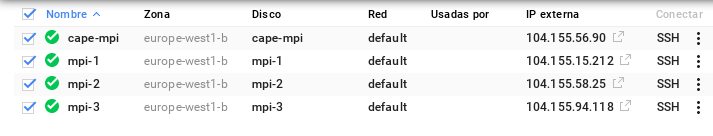
\includegraphics[scale=0.4]{maquinas.png}
  }
\end{frame}


\begin{frame}[fragile] 
  \frametitle{Resultados}
  \emph{
    Finalmente podemos observar los resultados obtenidos.
    \vspace*{30px}
    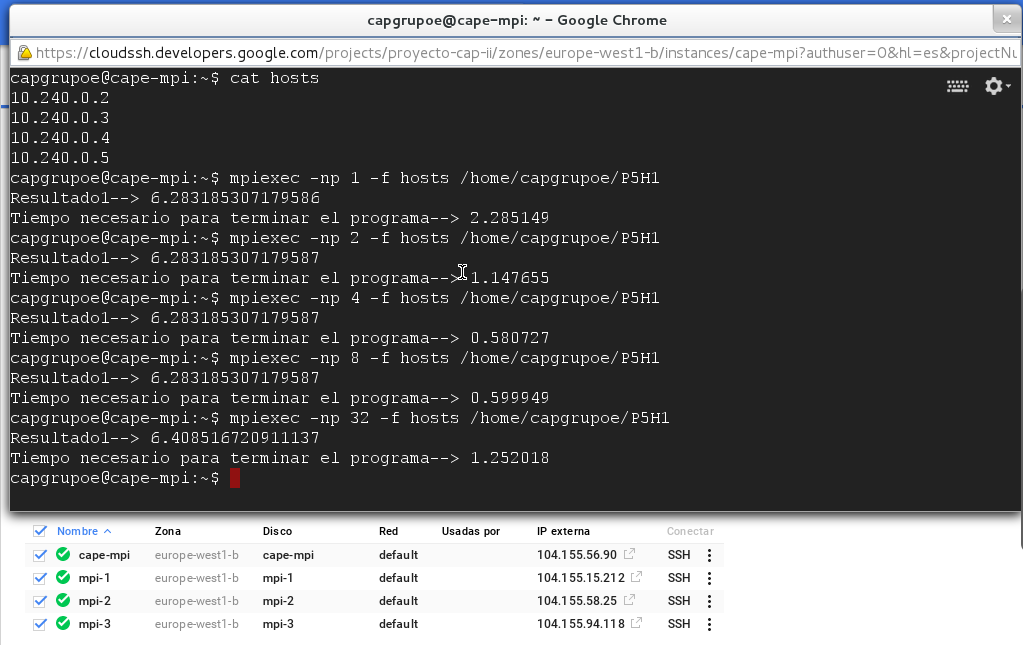
\includegraphics[scale=0.3]{resultado.png}
  }
\end{frame}

\end{document}
